% THIS IS SIGPROC-SP.TEX - VERSION 3.1
% WORKS WITH V3.2SP OF ACM_PROC_ARTICLE-SP.CLS
% APRIL 2009
%
% It is an example file showing how to use the 'acm_proc_article-sp.cls' V3.2SP
% LaTeX2e document class file for Conference Proceedings submissions.
% ----------------------------------------------------------------------------------------------------------------
% This .tex file (and associated .cls V3.2SP) *DOES NOT* produce:
%       1) The Permission Statement
%       2) The Conference (location) Info information
%       3) The Copyright Line with ACM data
%       4) Page numbering
% ---------------------------------------------------------------------------------------------------------------
% It is an example which *does* use the .bib file (from which the .bbl file
% is produced).
% REMEMBER HOWEVER: After having produced the .bbl file,
% and prior to final submission,
% you need to 'insert'  your .bbl file into your source .tex file so as to provide
% ONE 'self-contained' source file.
%
% Questions regarding SIGS should be sent to
% Adrienne Griscti ---> griscti@acm.org
%
% Questions/suggestions regarding the guidelines, .tex and .cls files, etc. to
% Gerald Murray ---> murray@hq.acm.org
%
% For tracking purposes - this is V3.1SP - APRIL 2009

\documentclass{acm_proc_article-sp}
\setlength{\parindent}{2em}

\begin{document}

\title{Anonymity Network: Cloud-based Onion Routing}

\numberofauthors{5} 

\author{
% 1st. author
\alignauthor
Fabian Gr�nbichler
% 2nd. author
\alignauthor
Klaus Krapfenbauer
% 3rd. author
\alignauthor
Thomas Hackl
\and  % use '\and' if you need 'another row' of author names
% 4th. author
\alignauthor 
Stefan Gamerith
% 5th. author
\alignauthor 
Milan Dzenovljanovic
}

\maketitle
\begin{abstract}
\textit{An anonymity network should enable users to access the public Web while, at the same time, hiding their identity on the Internet. 
Onion routing's anonymous connections are strongly resistant to traffic analysis and can be used through a socket connection. 
In an onion network, messages are encrypted and transmitted over a onion routers. Every onion router removes the layer of encryption, 
reads the routing instructions and sends the message to the next router in the chain where the same process is repeated. In the onion network chain
every router is aware just about existence of the previous end next node, and only the last node knows the content of a data.
Todays most used global onion routing network is Tor. Because of using a large number of volunteers, Tor faces a poor performance often.
Therefore as well as for benefits of Cloud computing (broad network access, resource pooling, rapid elasticity, ensured services), 
moving onion routing services into the "cloud" seems like a logical step.
This paper describes anonymous connections and their implementation using Cloud-based onion routing.
}
\end{abstract}

\terms{Security, Privacy}

\keywords{Anonymity networks, Onion routing, Cloud computing} 

\section{Introduction}
Anonymity networks enable users to communicate over the public Web while hiding their identity from one another.
Nevertheless, is Internet communication private? Greatest concerns today is preventing outsiders listening in on electronic
conversation. But \textit{traffic analysis} can also leak some sensitive information because encrypted messages can be tracked, revealing 
who is talking to whom. \cite{cite1}

Todays best and most popular tool for accessing the Internet anonymously is Tor. By taking the traffic through a sequence of nodes, 
Tor allows the traffic to appear to target from its last node, not from the user directly. Main disadvantage of Tor is that its relays are hosted 
by a volunteers all over the world. This volunteers mainly use private, consumer-grade ISP connections which often have limited bandwidth 
capacity, therefore Tor faces performance drops. \cite{cite2}

Moving onion routing services to the "cloud" will benefit with possibility to rotate between numbers of IP addresses as well as 
with large number of high-quality, high-bandwidth nodes. Great advantage of the "cloud" infrastructure  lays in its "elasticity".
By spawning new virtual machine instance in the "cloud" one can easily add or remove a new node to a "cloud". \cite{cite2}

Main goal of \textit{traffic analysis} is to discover participants of conversation, weather the participants are exchanging mails or 
user is just browsing the Web. Bearing this in mind, the \textit{anonymity networks} are developed to mislead the observers 
by making them difficult to identify informations, that are stored into the packet headers or in a track of encrypted payload, from the connection.
Thus, any information that carries identifying data must be sent through the \textit{anonymous  network}. Onion routing is implementation 
of \textit{anonymous network} that stands out with low latency and low overhead. Fundamentally, onion routing relays on Tor's protocol and 
provides two-way, real-time, connection-based communication that does not require the target to participate in the \textit{anonymity} protocol.
 All afore mentioned features together make anonymising communication on the Web easier. \cite{cite1} \cite{cite2}

\section{Onion routing}
\subsection{Overview}

In onion routing, user connects to a target over a sequence of machines called \textit{onion routers}, rather than connect directly to a target.
This way the \textit{originator} and the target remain anonymous to \textit{observer}. It is possible for the \textit{originator} to remain anonymous
to the target. In this case all informations that identifies the \textit{originator} have to be removed from the data stream before being sent over
the \textit{onion routing network}.

\subsection{Data transfer}
In the \textit{onion routing network} routers communicates over a TCP (it can be implemented on top of other protocols). The set of the 
\textit{onion routers} in a route is defined at very setup of the connection, when \textit{originator } creates an \textit{onion}, and each router knows only previous and next router  
along the route. An \textit{onion} is a layered data structure that encapsulates cryptographic informations such as the keys and cryptographic algorithms used 
during the data transfer. Along the route each \textit{onion router} uses its public key do decrypt the entire \textit{onion}. This way the identity of the next router 
along the route as well as embedded \textit{onion} is exposed. The \textit{onion router} ends the data to the next router and after the connection is established, the data can be sent in both directions. Using the keys and algorithms from the onion, the data is encrypted before it is sent from the originator. During the data transfer along the route, each \textit{onion router} 
removes one layer of encryption, like peeling an onion, so at the target the data arrives as a plain text. Because of the layered public key cryptography an \textit{onion} looks different 
to every \textit{onion router} along the connection. \cite{cite3}

\subsection{Overhead}
Because of the public key decryption, the most expensive calculation in the onion routing network is public-key cryptography, and it only takes place at the connection setup. In the data movement phase only the symmetric-key cryptography is used, which is much faster and can be as fast as ordinary link encryption. Delay in the data transfer depends on the number of the \textit{onion routers}. Overall, overhead in the \textit{onion routing} is sufficiently small. \cite{cite3}

\subsection{Formal Description}

Let say we have N number of routers, where each router have its own public (Su) and private (Sr) key. Public key is known to the \textit{originator} and private keys are known to the router. \cite{cite4}

As outlined before, \textit{onion routing protocol} relays on the public-key cryptography, therefore functions for encryption \textit{E[key](data)} and decryption \textit{D[key](data)} are needed. Key par in the public-key cryptography is generated in the way that data encrypted with public key Su can be decrypted only with private key Sr, and vice versa, i.e. \textit{D[Su](E[ Sr](data)) = data} and \textit{D[Sr](E[Su](data)) = data}. \cite{cite4}

When \textit{originator} wants to send informations over the \textit{onion routing network}, he sends a request to the \textit{onion proxy} and gets back the set of randomly chosen \textit{onion routers}, e.g. <4, 3, 5>. This means that information, which travels from the \textit{originator} to the \textit{target}, will be routed over this three routers respectively. The first router in the circuit\footnote{Circuit represents the logical connection between two nodes} is called \textit{entry node} and the last node is called \textit{exit node}. Before information is sent to the \textit{entry node}, \textit{onion proxy} creates an \textit{onion}, which in our case looks like: \textit{E[4u](3's IP address, E[3u]( 5' s IP address, E[5u](data)))}. The \textit{onion} is then forwarded to the \textit{entry node} (4). The \textit{entry node} decrypts the \textit{onion} with its private key, reads the IP address of the next node (3) and passes the the data to it where the same process is repeated. \cite{cite4}

It is possible that each router has a number of TCP connection to the other routers, and multiple circuits between two same nodes might use the same TCP connection.Therefore, every router needs to remember the association between two circuits. \cite{cite4}

When the circuit <4, 3, 5> is established it allows data to travel in both ways without including routing information. In the example above, when a response message from the \textit{target} arrives at the \textit{exit node} (5), (5) already know to which circuit and node (3) it should forward the information. (5) first encrypt the data it received from the \textit{target } with its private key and sends it to (3). (3) encrypts the data with its private key and sends it to (4). (4) does the same thing and passes the data to the \textit{onion proxy}. In order to read the original information, the \textit{onion proxy} decrypts the data it received from (4) as: \textit{D[4u](D[3u](D[5u]( encrypted onion)))}. \cite{cite4}

\begin{figure}
    \centering
    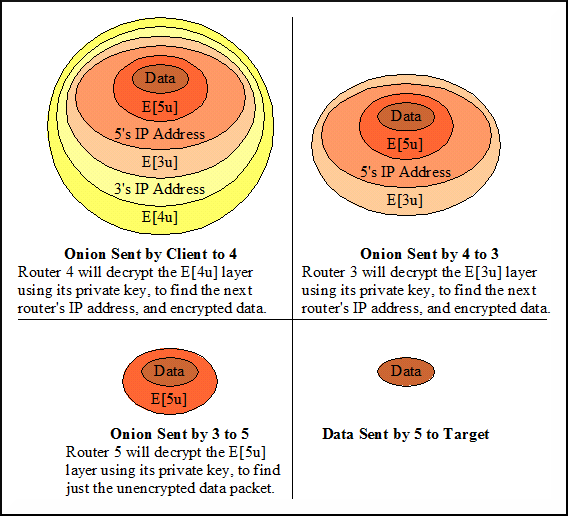
\includegraphics[width=0.5\textwidth]{anonion.png}
    \caption{Onion routing \cite{cite4}}
    \label{fig:onion_image}
\end{figure}

\subsection{Advanced considerations}

Thera are many ways to attack \textit{onion routing} systems today: Denial of Service (DoS) attacks, Distributed Denial of Service (DDoS) attacks, passive tracking analysis, active tracking analysis.\cite{cite4}

Making \textit{onion routing} secure is a research area that grows from day to day with plenty of different ideas. \cite{cite4}

\subsubsection{Denial of Service (Dos) and Distributed DoS} 

As stated in the The World Wide Web Security FAQ: \textit{Denial of Service (DoS) is an attack designed to render a computer or network incapable of providing normal services. The most common DoS attacks will target the computer's network bandwidth or connectivity. Bandwidth attacks flood the network with such a high volume of traffic, that all available network resources are consumed and legitimate user requests can not get through. Connectivity attacks flood a computer with such a high volume of connection requests, that all available operating system resources are consumed, and the computer can no longer process legitimate user requests.} \cite{cite5}

\textit{A Distributed Denial of Service (DDoS) attack uses many computers to launch a coordinated DoS attack against one or more targets.} \cite{cite5}

The best way to protect from the DoS attacks is to use digital currency like Hashcash\footnote{http://www.hashcash.org}. 

\subsubsection{Traffic Analysis}

The best way to protect from traffic analysis is to pay attention on the the size of the onion (all onions should be the same size) and make sure that information about timing on circuits is well hidden. \cite{cite4}

\section{Tor}
\subsection{Overview}

Tor is a second generation and the most sophisticated implementation of the \textit{onion routing}. First important upgrade that Tor brings is \textbf{perfect forward secrecy}: Tor now uses the \textit{"session" key} design, where the \textit{originator} negotiates with every node upon a \textit{"session" key} (shared secret). \textit{"Session" key} exchange protocol which Tor uses is called Diffie-Hellman\footnote{W. Diffie and M.E. Hellman, New directions in cryptography, IEEE Transactions on Information Theory 22 (1976), 644-654.} key exchange and keys that are generated during this exchange are valid only during the communication (depend on the circuit's lifetime). Public-key encryption is used only to establish connection. \cite{cite4} \cite{cite6}

\textbf{Congestion control}: Tor have an ability to detect congestion and sends less data until congestion goes down while maintaining anonymity. \cite{cite6}

\textbf{Directory servers}: Most reliable nodes act as \textit{directory servers}: they are able to control and monitor the chain nodes. Only \textit{directory servers} know the public key and IP address of the chain nodes, and every activ chain node has to register itself to the \textit{directory servers}. \cite{cite6}

\textbf{Leaky-pipe circuit topology}: \textit{Onion routing} allows only last node in the chain to be the \textit{exit node}. In Tor's implementation of the \textit{onion routing} this is changed allowing every node in the chain to be the \textit{exit node}. \cite{cite4}

\textbf{End-to-end integrity checking}: Tor verifies data integrity until it leaves the chain so that not a single node in the chain can change the contents of data cells. \cite{cite6}

\subsection{Design}

Tor's every \textit{onion router} connects over a TLS to every other \textit{onion router} in the network. Each user who uses Tor runs \textit{onion proxy} to maintain a circuits over the network, to communicate with \textit{directory server} and to maintain tho connections with user's applications.  \cite{cite6}

Each \textit{onion router} have a \textit{onion key} which is used to setup the circuit and \textit{identity key} which is used to register to the \textit{directory server} and to sign TLS certificates.  \cite{cite6}

Main unit of communication in Tor are fixed-size \textit{cells}.  \cite{cite6}

\subsection{Cells}

In Tor's design every \textit{cell} consists of header and payload and is fixed-size of 512 bytes. In the header of the \textit{cell} is a circuit identification number (CircID), which is used to identify the individual logical connection and instruction which tells what to do with the payload. We can distinguish two types of \textit{cells},  \textit{control cells} and  \textit{relay cells}.  \cite{cite6}

\textit{Control cells} consist of a commands: \textit{padding}, \textit{create} and \textit{created} (create a new circuit), \textit{destroy} (destroy a circuit) \cite{cite6}

\textit{Relay cells} are special as they tell the receiving node to forward the (encrypted) payload to the target. Content of the \textit{relay cells} is encrypted using AES. The commands of the \textit{relay cells} are: \textit{relay begin} (open a stream), \textit{relay data}, \textit{relay end} (close a stream), \textit{relay connected} (successful  relay begin), \textit{relay teardown} (close a broken stream), \textit{relay extend} (extend the circuit), \textit{relay extended} (acknowledge of the  \textit{relay extend}),  \textit{relay truncate} (terminate only part of the \textit{circuit}),  \textit{relay truncated} (acknowledge of the  \textit{relay truncate}),  \textit{relay sendme} (congestion control),  \textit{relay drop}.  \cite{cite6}

\begin{figure}
    \centering
    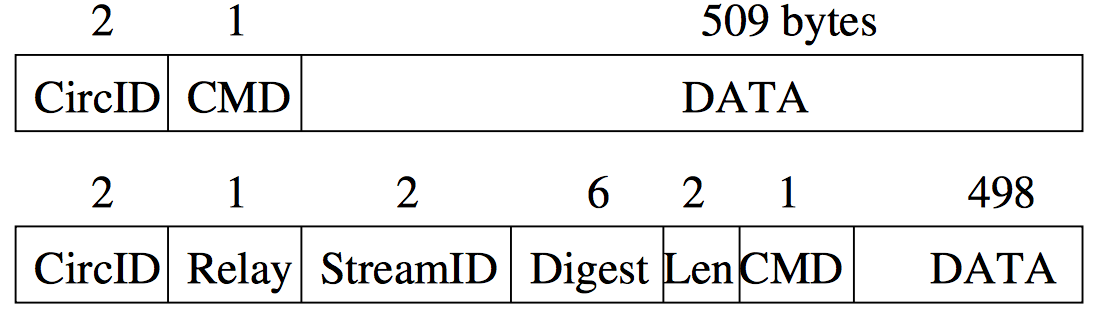
\includegraphics[width=0.5\textwidth]{cell.png}
    \caption{Cell \cite{cite6}}
    \label{fig:cell_image}
\end{figure}

\subsection{Construction of a circuit}

To create a \textit{circuit}, originator's \textit{onion proxy} sends a \textit{create cell} (with new CircID), which payload contains the first half of the Diffie-Hellman handshake, to the first node. First node responds with the \textit{created cell} containing its half of Diffie-Hellman and hash of their shared secret. At this point \textit{circuit} between this two nodes is created and they can send \textit{relay cells} to each other.  \cite{cite6}

To extend the circuit to the next node, originator's \textit{onion proxy} sends, along with the address of the second node and first half of the Diffie-Hellman handshake, to the first node a \textit{relay extend cell}. First node wraps the data in a \textit{create cell} (with new CircID) and passes it to the second node. Second node responds to the first node with the \textit{created cell}, along with its half of Diffie-Hellman and hash of the shared secret, which wraps the data in a \textit{relay extended cell} and passes to the originator. Now the \textit{circuit} is extended. \cite{cite6}

To extend the \textit{circuit} further, above mentioned protocol is repeated.

\begin{figure*}
    \centering
    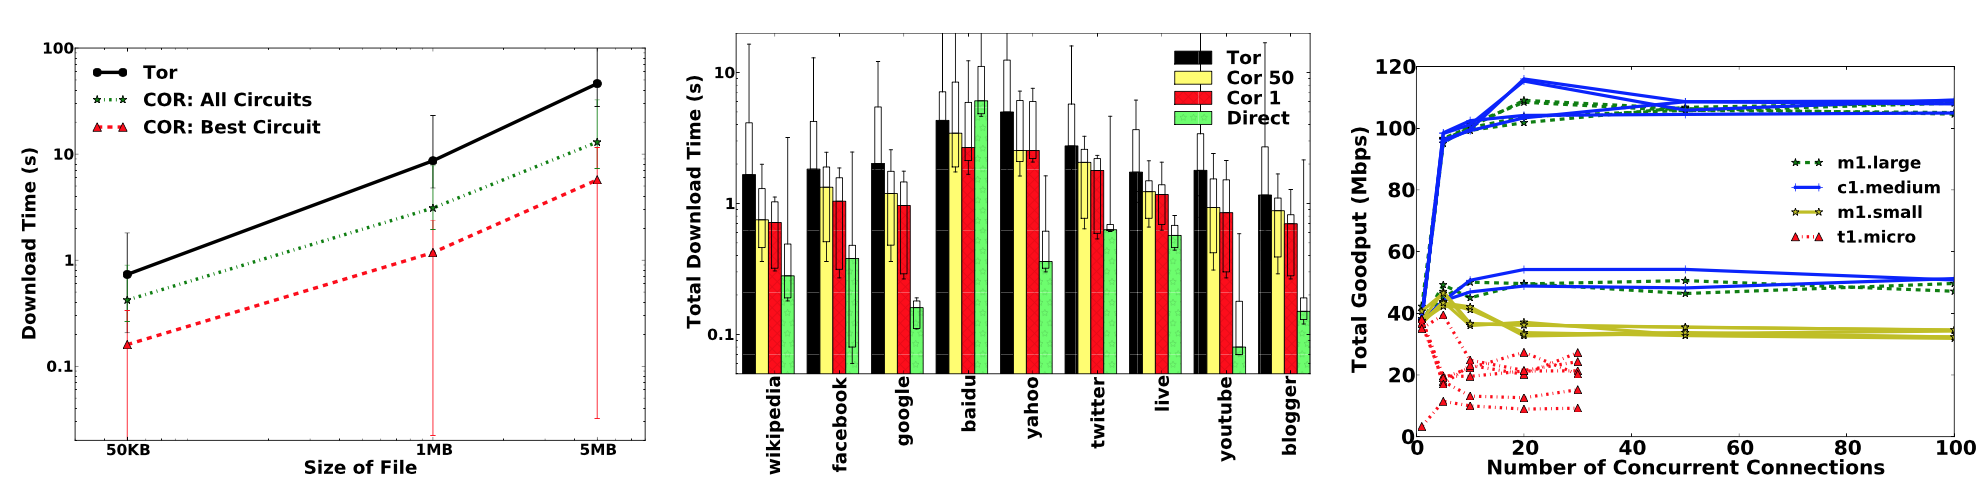
\includegraphics[width=1\textwidth]{evaluation.png}
    \caption{Evaluation \cite{cite2}}
    \label{fig:eval_image}
\end{figure*}

To tear down a \textit{circuit}, originator sends a \textit{destroy cell} which every node receives, closes that \textit{circuit} and passes the \textit{destroy cell} forward. Because of the incrementally nature of the \textit{circuit} building, it is possible to tear down a circuit incrementally. Originator can send a \textit{relay truncate cell} to one node in the circuit. That node passes the \textit{cell} forward and replays with the \textit{relay truncated cell}. This way originator is able to extend the circuit to different node. \cite{cite6}

\subsection{Opening and closing stream}

When originator wants to open a new connection to the target, he sends a request to the \textit{onion proxy} to open a stream. By sending the \textit{relay begin cell} to the \textit{exit node}, \textit{onion proxy} opens the stream. When the \textit{exit node} is connected to the target it sends the \textit{rally connected cell}. Now the \textit{onion proxy} can send data over the circuit in a \textit{relay data cell}. \cite{cite6}

We differentiate two types of cells for closing stream. When the stream is closed normally, one node sends a the \textit{relay end cell}, and the other side responds with its \textit{relay end cell}. For the stream that closes abnormally, the node next to the failed node sends a \textit{relay teardown cell}. \cite{cite6}

\section{Performance evaluation: Tor and Cloud-based Onion Routing}

This evaluation considers two experiments for comparison: \cite{cite2}
\begin{itemize}
  \item downloading single files (TorPref)
  \item downloading entire web sites
\end{itemize}

\textbf{Individual Files Download:}

For performance evaluation when downloading single files, Tor-supplied TorPref\footnote{https://metrics.torproject.org/tools.html} measurement tool is used. For experiments are used five \textit{cloud-based onion routing circuits} which were built over the US and EU datacenters, and five Tor circuits, randomly built by Tor. Three files of size 50KB, 1MB and 50MB, were downloaded repeating each download 100 times. The results are shown in the Figure 3 (left), and as you can see, the average \textit{cloud-based onion routing's} performance is better then Tor's.\cite{cite2}

\textbf{Downloading Web pages:}

For this purposes 10 \textbf{entire} home pages were downloaded using Tor, \textit{cloud-based onion routing} and a direct Internet connection, and each home page was downloaded 10 times in a row. For the \textit{cloud-based onion routing} downloads, two use cases were tested, one with the \textit{cloud-based onion routing relay} under load (serving 50 connections at the time) and serving just one connection at the time. In the Figure 3 (center) you can see that the \textit{cloud-based onion routing} is several times faster then Tor, although it is slower then direct access.\cite{cite2}

\textbf{Concurrent Users:}

Here is evaluated the number of concurrent users that one node can maintain. Also, for the purposes of this experiment, nodes of the different size (nodes differ in CPU, memory and I/O resources) from Amazon EC2 are evaluated. You can see that m1.large and c1.medium can maintain more then 100 concurrent users, while the t.micro has problem with handling 10 users. The results are shown in Figure 3 (right) where you can see that the two largest instances achieved speed between 50 Mbps and 120 Mbps.\cite{cite2}

\section{Conclusion}
The goal of \textit{onion routing} is to protect anonymity by hiding the destination of initiator. To fulfil its purpose \textit{onion routing} uses public-key encryption to encrypt the original data and to create an onion. During its way towards the target the onion will be decrypted at each hop. When a router peels one encrypted layer of it only sees the address of the next router in the circle. Since no one can see the full path, we can say that the communication is anonymous. \cite{cite4}

Because of elastic cloud infrastructure and powerful connectivity, \textit{cloud-based onion routing} introduces a new, higher level of implementation of \textit{onion routing} protocol. Also, \textit{cloud-based onion routing} brings additional level of protection against blocking, leaving censors with two options: allow the traffic or block all IP prefixes used by one cloud provider. Blocking all prefixes will cause a big damage: for example, Amazon EC2, hosted over a million instances with common IP prefixes in 2010.\footnote{Recounting EC2 One Year Later:
http://www.jackofallclouds.com/2010/12/recounting-ec2/} Preliminary surveys demonstrates that \textit{cloud-based onion routing} can be efficient, high performing and cost effective. \cite{cite2}.

\textit{Onion routing} is an applied solution for real anonymity problems but yet still a big research area. \cite{cite7}

\bibliographystyle{plain}

\balancecolumns


\begin{thebibliography}{9}

\bibitem{cite1}
  Michael D. Reed, Paul F. Syverson, David M. Goldschlag, Naval Research Laboratory,
  \emph{Anonymous Connections and Onion Routing}, 1998.
  
  \bibitem{cite2}
  Nicholas Jones, Matvey Arye, Jacopo Cesaero, Michael J. Freedman,
  \emph{Hiding Amongst the Clouds: A Proposal for Cloud-based Onion Routing}, Princeton University, 1998.
  
  \bibitem{cite3}
  Michael D. Reed, Paul F. Syverson, David M. Goldschlag, 
  \emph{Onion Routing for Anonymus and Private Internet Connection}, 1998.
  
    \bibitem{cite4}
  Marc O'Morian, Vladislav Titov, Wendy Verbuggen, 
  \emph{Onion Routing for Anonymus Communication},
  http://ntrg.cs.tcd.ie/undergrad/4ba2.05/group10/
  
      \bibitem{cite5}
  Lincoln Stein, John Stewart, 
  \emph{The World Wide Web Security FAQ: Securing against Denial of Service attacks},
  http://www.w3.org/Security/Faq/wwwsf6.html
  
    \bibitem{cite6}
  Roger Dingledine, Nick Mathewson, Paul Syverson, 
  \emph{Tor: The Second-Generation Onion Router}.
  
  \bibitem{cite7}
Paul F. Syverson,  Naval Research Laboratory,
  \emph{A Peel of Onion}.

\end{thebibliography}

\end{document}
